\section{Algoritmo X (nome do algoritmo da solução)}
\label{sec-complexidade-algoritmo}

Nesta seção são descritas as etapas da ACS aplicado ao problema anteriormente apresentado, foi utilizado a ferramenta \textit{Google Colab} para a implementação do código em \textit{Python} por permitir o desenvolvimento simultâneo de dois desenvolvedores, o que favore. Para facilitar a implementação do algoritmo, decidiu-se organizá-lo da seguinte forma:
\begin{enumerate}
    \item Importação e inicialização;
    \item Construção da solução por cada formiga naquela iteração;
    \item Calculo de custo de coancestralidade;
    \item Calculo de valor genético dos animais;
    \item Atualização da melhor solução encontrada;
    \item Evapora e deposita os feromônios conforme o desempenho das soluções;
\end{enumerate}
\vspace{1em}

\subsection*{1) Inicialização e Preparação das Estruturas}
Esse trecho de código implementa a primeira etapa do processo, responsável por carregar, validar e padronizar os arquivos de entrada utilizados pelo algoritmo ACS. Inicialmente, são importadas bibliotecas essenciais para manipulação de dados, operações matemáticas, controle de arquivos e entrada do usuário. Em seguida, o código lê automaticamente o arquivo contendo informações de coancestralidade diretamente de uma URL do \textit{GitHub}, normaliza seus nomes de colunas e garante que elas sigam o formato padrão esperado pelo algoritmo. Esse processo inclui tratamento de erros e  detecção de suporte ao ambiente utilizado. Após a seleção, o arquivo é lido com segurança; caso a leitura falhe, o programa é encerrado para evitar inconsistências futuras. Por fim, as colunas do arquivo de índices são padronizadas, convertendo nomes para minúsculas, removendo espaços e renomeando-as para os identificadores esperados. Essa padronização garante que, independentemente da origem ou formatação original do arquivo, os dados estarão consistentes para as etapas seguintes do algoritmo.

\begin{verbatim} 
start_time = time.time()

para iteracao em 0 .. NUM_ITERACOES:
    criar lista solutions_in_iteracao
    para cada formiga:
        caminho_formiga = []
        uso_machos = dicionario contador zerado
        valid_path = True
\end{verbatim}
\vspace{1em}

\subsection*{2) Construção da Solução por Cada Formiga}
Essa etapa identifica automaticamente os machos e fêmeas presentes nos dados de coancestralidade. Para isso, cada código no formato machoID\_femeaID é dividido para extrair separadamente os identificadores, que são armazenados em conjuntos para garantir unicidade. Após processar todas as entradas, os conjuntos são convertidos em listas ordenadas, permitindo determinar o número total de machos e fêmeas utilizados no problema.

\begin{verbatim}
para cada fêmea i_f:
    probabilidades = []
    candidatos_validos = []

    para cada macho i_m:
        se uso_machos[i_m] >= MAX_USO_MACHO:
            prob = 0
        senao:
            t = tau[i_f, i_m] ** ALPHA
            n = heuristica[i_f, i_m] ** BETA
            prob = t * n
            adicionar i_m a candidatos_validos

        armazenar prob nas probabilidades

    denom = soma(probabilidades)

    se denom > 0:
        normalizar probabilidades
        escolha_macho_idx = escolha aleatória ponderada
    senao:
        se candidatos_validos vazio: descartar caminho
        escolha_macho_idx = escolha aleatória simples

    registrar (i_f, escolha_macho_idx) no caminho
    incrementar uso_machos[escolha_macho_idx]
\end{verbatim}
\vspace{1em}

\subsection*{3) Cálculo da Coancestralidade da Solução}
A etapa de cálculo da coancestralidade tem como objetivo transformar os dados brutos presentes no dataframe em uma matriz (ou estrutura equivalente) que permite consultar rapidamente o coeficiente de parentesco entre qualquer par macho–fêmea. Embora o trecho de código não tenha sido mostrado, o funcionamento típico dessa fase — e o papel que ela cumpre dentro do algoritmo — pode ser descrito da seguinte forma:

\begin{verbatim}
cost_coancestralidade = 0
pares_reais = converter índices (i_f, i_m) para (id_m, id_f)

para i em 0..n_pares:
    para j em i+1 .. n_pares:
        cost += coancestralidade_dict[(par_i, par_j)]
\end{verbatim}
\vspace{1em}

\subsection*{4) Cálculo da Soma dos Índices Genéticos}
Esta etapa calcula a partir dos índices genéticos de machos e fêmeas. Primeiro, os índices individuais são extraídos e combinados em todas as possíveis duplas macho–fêmea, somando cada par e dividindo por dois para obter um valor médio representativo. Em seguida, a matriz resultante é verificada para identificar valores zero ou negativos, que prejudicariam o comportamento do ACO; caso existam, toda a matriz é normalizada ao adicionar o módulo do menor valor mais 1, garantindo que todos os elementos sejam positivos. O resultado final é armazenado que será utilizada como componente heurística na construção das soluções pelas formigas.

\begin{verbatim}
sum_indice_genetico = 0

para cada par (i_f, i_m) no caminho:
    sum_indice_genetico += matriz_indices_reais[i_f, i_m]
\end{verbatim}
\vspace{1em}

\subsection*{5) Atualização da Melhor Solução Global}
Esta etapa transforma os dados brutos de coancestralidade em uma estrutura eficiente para consulta e coleta um parâmetro essencial do ACO. Primeiro, cada identificação no formato macho\_fêmea é convertida em uma tupla numérica, e um dicionário é criado para armazenar rapidamente o coeficiente de coancestralidade entre qualquer par de casais — incluindo ambas as ordens, garantindo acesso simétrico. Esse dicionário será usado pelo algoritmo para calcular o impacto genético das combinações durante a otimização. Em seguida, o código apresenta um menu simples para que o usuário escolha o limite máximo de uso dos machos, definindo uma das principais restrições do problema antes de iniciar o processo de busca do ACO.

\begin{verbatim}
se cost < best_cost:
    atualizar best_cost
    atualizar best_solution
    atualizar best_index_sum

senao se cost == best_cost e sum_indice_genetico > best_index_sum:
    atualizar best_solution e índices
\end{verbatim}
\vspace{1em}

\subsection*{6) Evaporação e Deposição de Feromônio}
Esse trecho implementa o núcleo do algoritmo de Otimização por Colônia de Formigas responsável por buscar a melhor combinação entre machos e fêmeas. O processo começa inicializando parâmetros como número de formigas, iterações, importância do feromônio \(\alpha\) , da heurística \(\beta\)\, taxa de evaporação e matriz de feromônios. A cada iteração, cada formiga constrói uma solução completa escolhendo um macho para cada fêmea com base em probabilidades que dependem tanto do feromônio acumulado quanto da heurística genética sempre respeitando o limite de uso dos machos. Ao final de cada construção, a solução é avaliada por dois critérios: minimizar a coancestralidade e maximizar o índice genético total. A melhor solução encontrada é mantida, e os feromônios são atualizados: evaporam globalmente e aumentam proporcionalmente à qualidade das soluções construídas. Esse ciclo se repete por várias iterações, guiando gradualmente o algoritmo para combinações mais promissoras até alcançar a melhor configuração encontrada dentro do número definido de iterações.

\begin{verbatim}
tau *= (1 - EVAPORATION)

para cada solucao em solutions_in_iter:
    custo = sol[custo]
    se custo <= 0.0001: custo = 0.0001
    delta = Q / custo

    para cada par (i_f, i_m) da solução:
        tau[i_f, i_m] += delta
\end{verbatim}
\vspace{1em}

\subsection*{7) Impressão dos Resultados e Relatório Final}
Essa etapa é responsável por apresentar e validar o resultado final encontrado pelo algoritmo ACO. Primeiro, o código percorre a melhor solução identificada, reconstrói cada par fêmea–macho e calcula o índice genético correspondente, armazenando tudo em uma lista organizada para análise. Ele imprime apenas os dez primeiros pares para visualização, informando caso haja mais resultados. Em seguida, contabiliza quantas vezes cada macho foi usado e calcula estatísticas finais importantes: custo mínimo de coancestralidade, soma total dos índices genéticos, média dos índices da progênie e o macho mais utilizado. Por fim, verifica se a restrição de uso máximo por macho foi respeitada e informa o status geral da solução; caso nenhuma solução tenha sido encontrada, exibe um aviso de falha crítica.

\begin{verbatim}
end_time = time.time()
print("Tempo total:", end_time - start_time)

se best_solution existe:
    para cada par (i_f, i_m) na solução:
        imprimir IDs e índice genético

    gerar estatísticas gerais:
        - melhor custo
        - soma de índices
        - média da prole
        - machos mais usados
        - verificação da restrição de uso

senao:
    imprimir "FALHA CRÍTICA: Nenhuma solução encontrada."
\end{verbatim}

Após a implementação do algoritmo foi realizado uma análise para avaliar o custo dominante da análise assintótica, onde foi evidenciado dois custos principais:
\begin{itemize}
    \item Cálculo da coancestralidade, onde a cada iteração o custo é \(O((i\_j)^2)\);
    \begin{verbatim}
        for i in range(n_pares):
            for j in range(i + 1, n_pares):
                coancest_dict += coancest_dict.get((par_a, par_b), 0.0)
    \end{verbatim}
    \item Custo de construir o caminho da formiga, onde para cada fêmea é avaliado um macho, construindo um custo de \(O(i\ *\ j)\), que, dependendo do contexto, pode vir a ser \(O((i\_j)^2)\) dependendo do número de formigas.
    \begin{verbatim}
        for i_f in range(num_femeas):
            probabilidades = []
            candidatos_validos = []

            for i_m in range(num_machos):
                if uso_machos[i_m] >= MAX_USO_MACHO:
                prob = 0.0
            else:
                t = tau[i_f, i_m] * ALPHA
                n = matriz_heuristica_eta[i_f, i_m] * BETA
                prob = t * n
                candidatos_validos.append(i_m)
            probabilidades.append(prob)
    \end{verbatim}
\end{itemize}
Dessa forma, é possível observar que a complexidade final do algoritmo também deve incluir \(I\) iterações e \(n\) formigas, além dos \(i\_j\)\ pares, assim, o custo total leva em conta é :

\begin{center}
    \(O(I\ *\ A\ *\ (n^2\ +\ i\ *\ j))\)
\end{center} 
Que pode ser simplificado em, considerando que o termo dominante do parêntese é o \(n^2\):
\begin{center}
    \(O(I\ *\ A\ *\ n^2)\)
\end{center}
\vspace{1em}
\section{Análise de Complexidade Experimental}

Além da análise teórica da complexidade, foi conduzida uma avaliação empírica do custo computacional do algoritmo ACO. Para isso, variou-se isoladamente o número de formigas e o número de iterações, registrando-se o tempo total de execução em cada configuração. É importante destacar que esses gráficos não representam a convergência do algoritmo, mas sim sua escalabilidade temporal.

A Figura~\ref{fig:tempo_formigas} apresenta a relação entre o tempo de execução e o tamanho da população de formigas. Observa-se um crescimento aproximadamente linear, o que confirma o comportamento esperado da complexidade, uma vez que cada formiga constrói uma solução completa em cada iteração. Assim, aumentar o número de formigas aumenta diretamente o custo computacional.

\begin{figure} [htpb]
    \centering
    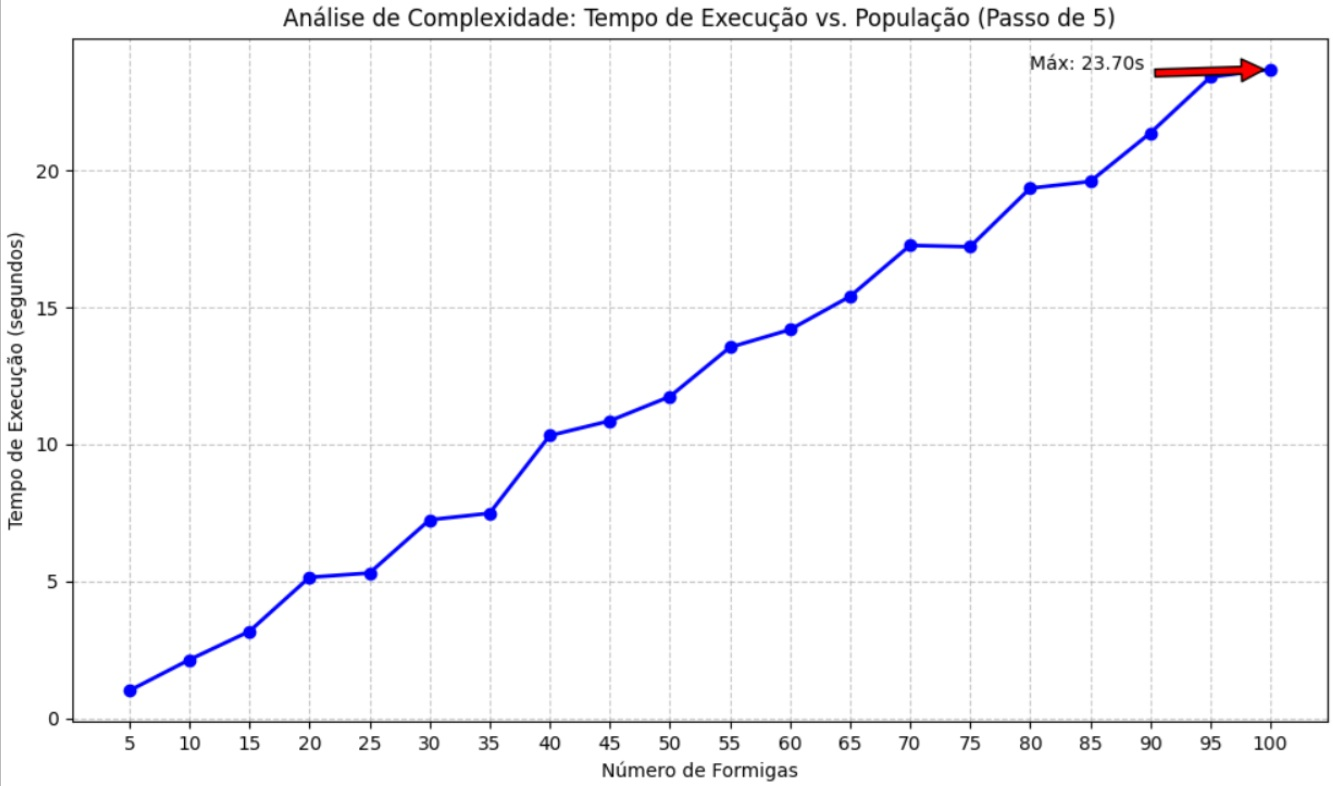
\includegraphics[width=0.75\linewidth]{Imagens/num_formigas.jpg}
    \caption{Tempo de execução em função do número de formigas.}
    \label{fig:tempo_formigas}
\end{figure}

Já a Figura~\ref{fig:tempo_iteracoes} mostra o tempo de execução em função do número de iterações. Também se verifica crescimento linear, uma vez que cada iteração envolve a construção de todas as soluções e a atualização global dos feromônios. Portanto, o custo cresce proporcionalmente ao número de ciclos da colônia.

\begin{figure} [htpb]
    \centering
    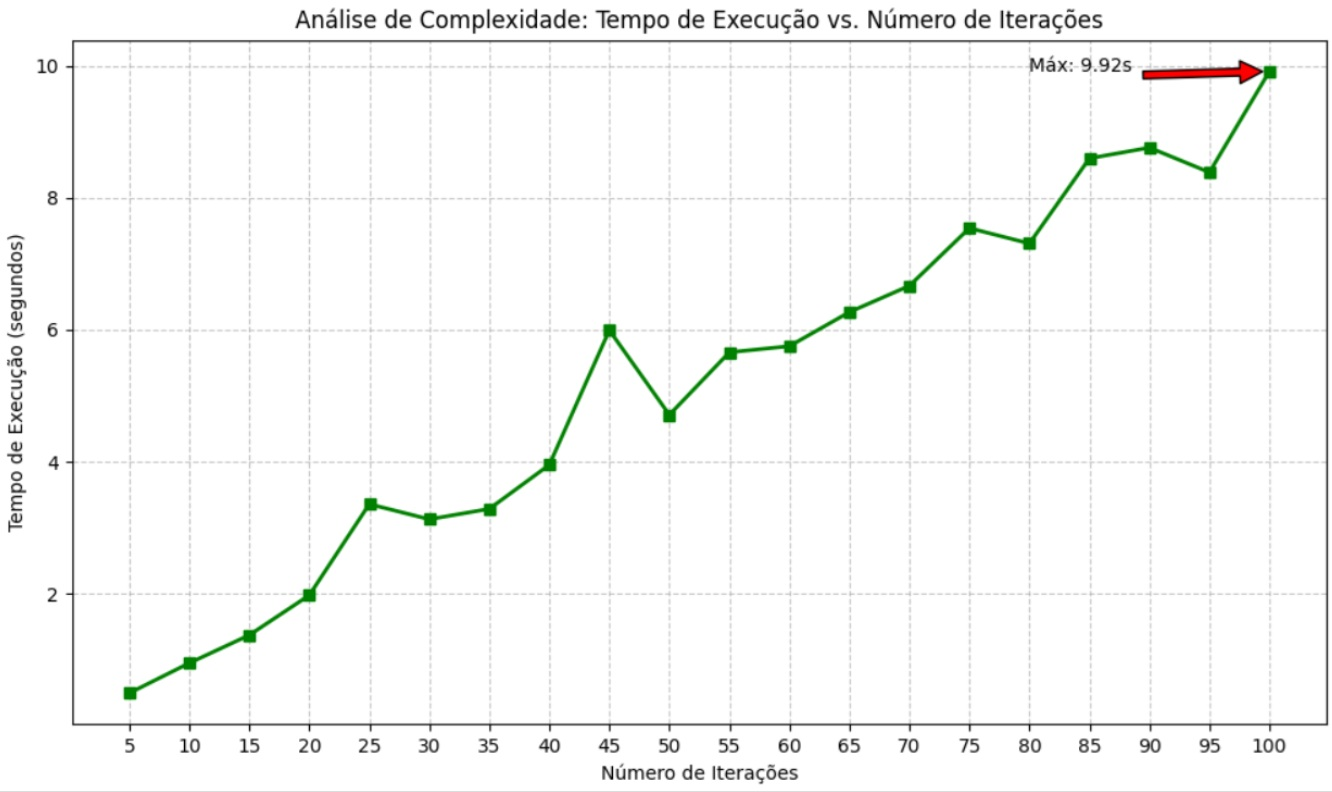
\includegraphics[width=0.75\linewidth]{Imagens/num_iteracoes.jpg}
    \caption{Tempo de execução em função do número de iterações.}
    \label{fig:tempo_iteracoes}
\end{figure}
